\sectionquestion{Learning Theory}

\begin{parts}
\begin{comment}
\part[5] Consider a dataset of points $\{(x^{(i)}, y^{(i)})\}$ where linear regression is applied to model the data points. Let $c^*$ be the unknown, true function that models the distribution of points.
\begin{subparts}
    \subpart[1] Describe the hypothesis space $\mathcal{H}$ for this model
    \fillwithlines{3em}
    \begin{soln}
        All linear functions
    \end{soln}
    \subpart[2] Is this a Realizable or Agnostic setting? Explain why.
    \fillwithlines{6em}
    \begin{soln}
        Agnostic. It's possible $c^* \notin \mathcal{H}$ because the data cannot be modeled with a linear function
    \end{soln}
    \subpart[2] Is this hypothesis space Finite or Infinite? Explain why.
    \fillwithlines{6em}
    \begin{soln}
        Infinite. All linear functions
    \end{soln}
\end{subparts}
\begin{qauthor}
    Removed by Henry: I confess I'm not too sure what is being tested by this question but it seems to be mixing the ideas of lienar regression and classification somewhat problematically...
\end{qauthor}
\end{comment}

\part[2] \textbf{Select all that apply:} Recall the sample complexity bound for the finite, realizable case:
\begin{quote}
    Given a finite hypothesis set $\mathcal{H}$ s.t. $c^* \in \mathcal{H}$, if the number of training data points satisfies $M \geq \frac{1}{\epsilon} \bigg( \ln(|\mathcal{H}|) + \ln\Big(\frac{1}{\delta}\Big) \bigg)$ then with probability at least $1-\delta$, all $h \in \mathcal{H}$ with $\hat{R}(h) = 0$ have $R(h) \leq \epsilon$.
\end{quote}
In this setting, if you are given $M = \frac{1}{2\epsilon} ( \ln(|\mathcal{H}|) + \ln (\frac{1}{\delta}) )$ labelled training data points, which of the following statements hold with probability at least $1 - \delta$?
{%
    \checkboxchar{$\Box$} \checkedchar{$\blacksquare$} % change checkbox style locally
    \begin{checkboxes}
        \choice All $h \in \mathcal{H}$ with $R(h) > 2\epsilon$ have $\hat{R}(h) > 0$
        \choice No $h \in \mathcal{H}$ with $\hat{R}(h) = 0$ have $R(h) > 2\epsilon$
        \choice All $h \in \mathcal{H}$ with $\hat{R}(h) = 0$ have $R(h) \leq \frac{\epsilon}{2}$
        \choice No $h \in \mathcal{H}$ with $R(h) > \frac{\epsilon}{2}$ have $\hat{R}(h) = 0$
        \choice None of the above
    \end{checkboxes}
}
\begin{soln}
    A, B
\end{soln}
\begin{qauthor}
    Henry (adapted from Alex's S23 question), Define PAC and explain what it means to be approximately correct and what occurs with high probability
\end{qauthor}

\part[1] \textbf{True or False:} Suppose you have two hypothesis sets $\mathcal{H}_1$ and $\mathcal{H}_2$. If $\mathcal{H}_1 \subset \mathcal{H}_2$ i.e., $\mathcal{H}_1$ is a \emph{strict} subset of $\mathcal{H}_2$, then the VC-dimension of $\mathcal{H}_1$ is \emph{strictly} less than the VC-dimension of $\mathcal{H}_2$. Briefly justify your answer in 1-2 concise sentences. 
\begin{checkboxes}
    \choice True 
    \choice False
\end{checkboxes}
\fillwithlines{7em}
\begin{soln}
    False, they could be equal to one another.
\end{soln}
\begin{qauthor}
    Henry
\end{qauthor}


\newpage
\part[2] \textbf{Select all that apply:} Which of the following hypothesis sets can shatter the dataset of four points shown below? 
\begin{center}
    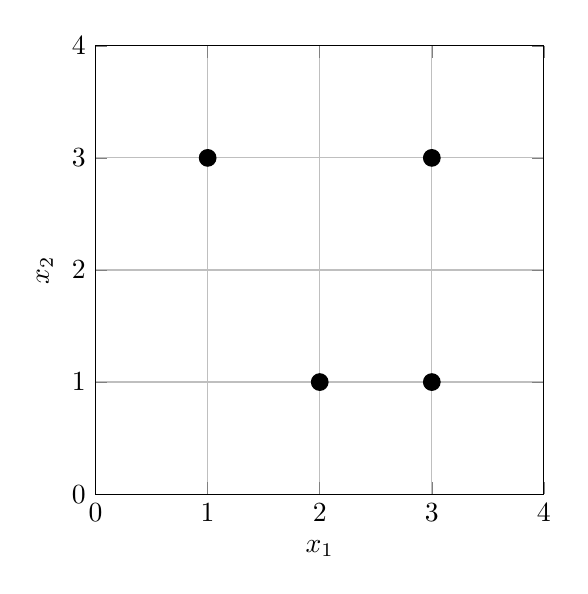
\begin{tikzpicture}
    \begin{axis}[
        scale=1, axis equal image, mark options={scale=1.5},
        xmin=0, xmax=4, xtick={0,...,4},
        ymin=0, ymax=4, ytick={0,...,4},
        grid=major, xlabel=$x_1$, ylabel=$x_2$]
        \addplot[scatter,
            only marks,
            point meta=explicit symbolic,
            scatter/classes={
                a={mark=*,black}
            }
        ] table [meta=label] {
            x y label
            1 3 a
            2 1 a
            3 1 a
            3 3 a
        };
    \end{axis}
    \end{tikzpicture} 
\end{center}
{%
    \checkboxchar{$\Box$} \checkedchar{$\blacksquare$} % change checkbox style locally
    \begin{checkboxes}
        \choice All linear decision boundaries
        \choice All axis-aligned rectangles i.e., rectangles where each side is parallel to either the x-axis or the y-axis
        \choice All \emph{squares} (note: these do not have to be axis-aligned)
        \choice All decision trees over $x_1$ and $x_2$
        \choice None of the above
    \end{checkboxes}
}
\begin{soln}
    C, D
\end{soln}
\begin{qauthor}
    Henry, heavily inspired by UNKNOWN
\end{qauthor} 


\part[2] \textbf{Select One:} What is the VC-dimension of a 1-nearest neighbor classifier on $D$-dimensional inputs? Assume the distance metric is Euclidean distance. Briefly justify your answer in 2-3 concise sentences. 
\begin{checkboxes}
    \choice $1$
    \choice $2$
    \choice $D$
    \choice $D+1$
    \choice $\infty$
\end{checkboxes}
\fillwithlines{6em}
\begin{soln}
    E; for any set of $N$ data points, a 1-NN can generate all possible labelings. To see this, fix an arbitrary labeling, use the original set of $N$ points as the training dataset and set the labels to be the desired labeling. 
\end{soln}
\begin{qauthor}
    Henry, heavily inspired by UNKNOWN
\end{qauthor} 

\begin{comment}
\begin{subparts}
    \subpart[]\textbf{Short answer:} Given a rectangular classifer (defined by four corner points), where all points inside the rectange are "+" and all points outside are "-", is it possible to shatter this dataset? Why or why not?
    \fillwithlines{6em}
    \begin{soln}
        Yes, we can rotate the rectangle (so it sits diagonally) to correctly classify $(1, 3), (3,1)$ as both being positive and the rest negative. Also, $(2,1), (3, 3)$ as both being positive and the rest negative.
    \end{soln}
    
    \subpart[]\textbf{Select one:} Using the same dataset above, what is the VC-dimension of a KNN classifier where $k=1$?
    \begin{checkboxes}
     \choice $1$ 
     \choice $2$
     \choice $3$
     \choice None of the above
    \end{checkboxes}
    \begin{soln}
        None of the above (Infinity)
    \end{soln}
\end{subparts}

\part[2] \textbf{Select all that apply:} Consider a finite-sized set $\Sc$ consisting of all unique binary feature vectors of length $M$. Let $\Hc_d$ be the hypothesis class of decision trees of maximum depth $d$, where each split is binary on the 0/1 values of a single feature. In which of the following cases could $\Hc_d$ shatter $\Sc$?
    {%
    \checkboxchar{$\Box$} \checkedchar{$\blacksquare$} % change checkbox style locally
    \begin{checkboxes}
     \choice $M$ = 1, $d$ = 1 \hspace{6em} (Reminder: depth $d$ is the length of the
     \choice $M$ = 2, $d$ = 2 \hspace{6em} longest path from the root to a leaf.)
     \choice $M$ = 2, $d$ = 3
     \choice $M$ = 3, $d$ = 2
     \choice None of the above 
    \end{checkboxes}
    }
    \begin{soln}
        A, B, C
    \end{soln}
    \begin{qauthor}
        Tanvi, Check if students understood the concept of shattering a classifier. I also have an idea to complicate this further by bringing in VC dimension if it's too easy.
    \end{qauthor}
    \begin{qtester}
     Good question! there is a lot to understand in order to figure this out!
    \end{qtester}


\part[2] \textbf{Select all that apply:} Recall the PAC learning bound for the finite, realizable case:
%
\textit{
For a finite hypothesis set $\mathcal{H}$ s.t. $c^* \in \mathcal{H}$, if the number of training data points satisfies 
$N \geq \frac{1}{\epsilon} \bigg( \ln(|\mathcal{H}|) + \ln\Big(\frac{1}{\delta}\Big) \bigg)$
then with probability at least $1-\delta$, all $h \in \mathcal{H}$ with $\hat{R}(h) = 0$ have $R(h) \leq \epsilon$.
}

If instead, $N = \frac{1}{2} \cdot \frac{1}{\epsilon} ( \ln(|\mathcal{H}|) + \ln (\frac{1}{\delta}) )$, which of the following hold with probability at least $1 - \delta$?
{%
    \checkboxchar{$\Box$} \checkedchar{$\blacksquare$} % change checkbox style locally
    \begin{checkboxes}
     \choice No $h \in \mathcal{H}$ with zero training error can have $R(h) \leq \epsilon$.
     \choice At least one $h \in \mathcal{H}$ with zero training error has $R(h) \leq \epsilon$.
     \choice All $h \in \mathcal{H}$ with zero training error have $R(h) \leq 2\epsilon$.
     \choice At least one $h \in \mathcal{H}$ with zero training error has $R(h) > \epsilon$.
     \choice None of the above
    \end{checkboxes}
}
\begin{soln}
    C
\end{soln}
\begin{qauthor}
    Alex, Define PAC and explain what it means to be approximately correct and what occurs with high probability
\end{qauthor}


\part[1] \textbf{Short answer:} In practice, training error $\widehat{R}(h)$ tends to decrease as we increase model complexity (e.g., VC-dimension). Describe in detail how the true error $R(h)$ is related to model complexity.
    \fillwithlines{6em}
    \begin{soln}
        True error tends to decrease with model complexity to a point, after which it starts increasing.
    \end{soln}
    \begin{qauthor}
    Emaan, Learning Objective: Theoretically justify regularization. Lecture 16, slide 29 (Learning Theory and Model Selection).
    \end{qauthor}
        
\part[1] \textbf{Short answer:} During training, describe one technique we can use to limit model complexity while still achieving good true error in the end. For full credit, clearly identify how this technique limits model complexity as represented by VC Dimension. 
    \fillwithlines{6em}
    \begin{soln}
        We should use a regularizer to tradeoff between complexity and error. Regularization reduces the VC dimension, allowing us to find the best tradeoff point.
    \end{soln}
    \begin{qauthor}
    Emaan, Learning Objective: Theoretically justify regularization. Lecture 16, slide 29 (Learning Theory and Model Selection).
    \end{qauthor}    
\end{comment}

\end{parts}